\documentclass{bioinfo}
\usepackage{appendix}
\usepackage{fixltx2e}
% \usepackage{hyperref}
\copyrightyear{2010}
\pubyear{2010}

\begin{document}
\firstpage{1}

\newtheorem{theorem}{Theorem}[section]
\newtheorem{lemma}[theorem]{Lemma}
\newtheorem{proposition}[theorem]{Proposition}
\newtheorem{corollary}[theorem]{Corollary}

\newenvironment{definition}[1][Definition]{\begin{trivlist}
\item[\hskip \labelsep {\bfseries #1}]}{\end{trivlist}}
\newenvironment{example}[1][Example]{\begin{trivlist}
\item[\hskip \labelsep {\bfseries #1}]}{\end{trivlist}}
\newcommand{\todo}[1]{\textcolor{red}{#1}}
\newcommand{\update}[1]{\textcolor{blue}{#1}}
\newcommand{\old}[1]{\textcolor{green}{#1}}
\newenvironment{remark}[1][Remark]{\begin{trivlist}
\item[\hskip \labelsep {\bfseries #1}]}{\end{trivlist}}
\title[NETGEM]{NETGEM: Network Embedded analysis of Temporal Gene Expression using Mixtures}
%\title[short Title]{Analysis of temporal gene expression using mixture models}
\author[Sample \textit{et~al}]{Vinay Jethava\,$^{1}$, Torbjorn Karfunkel$^{2}$, Chiranjib Bhattacharyya\,$^{1}$, Devdatt Dubhashi$^{2}$,Goutham N.
  Vemuri$^{3}$\footnote{to whom correspondence should be addressed}}
\address{$^{1}$Computer Science and Automation Department, Indian Institute of Science,
Bangalore, INDIA\\
$^{2}$Department of Computer Science, Chalmers University of
  Technology, G\"oteborg, SWEDEN\\
$^{3}$Systems Biology, Department of Chemical and Biological Engineering, Chalmers University of
Technology, G\"oteborg, SWEDEN\\
}

\history{Received on XXXXX; revised on XXXXX; accepted on XXXXX}
\editor{Associate Editor: XXXXXXX}

\maketitle

\begin{abstract}
\section{Motivation}

\section{Results}

\section{Availability:}
The source code for NETGEM is available from http://129.16.106.142/

\section{Contact:} goutham@chalmers.se 
\end{abstract}

\section{Introduction}
% This paper studies problem of the temporal rewiring in a genetic
% network based on the observed microarray expression data. 

Microarrays have become a routine tool in biological enquiry, geared to measure 
global gene expression in response to genetic or 
environmental perturbations. Gene expression microarrays present a
snapshot of the transcriptional profile of all the genes at the time
of measurement. The outcome is a
vast amount of data, which has been analyzed using several statistical
methods including hierarchical clustering~\citep{Eisen98}, $k$-means
clustering~\citep{Tavazoie99}, self organizing
maps~\citep{Tomoya99som}, singular value decomposition~\citep{DBLP:journals/bioinformatics/RifkinK02}.  The key focus of the methods has 
been clustering of genes that have similar expression profile, based
on the assumption that co-expressed genes are likely to be regulated. 
An inherent drawback of the clustering approaches is their
unsuitability in the analysis of temporal expression data.  

% Time
% course data on gene expression provides substantial insight into the
% dynamics of transcriptional regulation, such as sequential events in
% invoking transcriptional response, any time lag in the process and
% relate the amplitude of the signal to different perturbations
% \textcolor{red}{[general REF on time series]}. Since time series data
% have a natural temporal ordering, using conventional methods to
% analyze time series data will fail to capture the internal structure
% of the data. Moreover, these methods also fail to consider that
% observations closer in time are likely to be closer than temporally
% distant observations. Unfortunately, the traditional framework of time
% series analysis cannot be used to analyze temporal gene expression
% data due to the small number of observations (time points), owing to
% cost and/or biological limitations. 

This has led to growing interest towards development of dedicated
algorithms to handle the temporal data. One of the key challenges
is the small number of observations~(time points), owing to cost
and/or biological limitations.  Several methods have been
investigated including significance
analysis~\citep{Tusher01sam,Leek06EDGE}, autoregressive curves based
model~\citep{Ramoni02cluster}, 
hidden markov models (HMM)~\citep{DBLP:conf/ismb/SchliepSS03,citeulike:1069055}, mixture 
models~\citep{DBLP:conf/ismb/SchliepSS04,DBLP:journals/bioinformatics/CostaSS05},
clustering methods~\citep{Ernst06STEM}, association
rules~\citep{Nam2009}. A review of the methods is available in
\cite{Androulakis2007}. However, the previous methods 
assume an time-invariant network topology, such as the protein-protein
interaction network or the genetic network inferred from microarray
data. 

\cite{Song09KELLER} first investigated the problem of discovering the
temporally-varying interaction networks based on local neighbourhood selection
with $l1$-regularization to obtain sparse networks. The analysis assumes a
smooth variation in the network interactions strengths to overcome the
unreliability of results due to the small number of observations
available in most biological experiments. 

This paper focusses on a different version of the rewiring problem. We
assume that the interactions network is known with a high degree of
confidence\todo{[BIOREF NEEDED]}.  The observed expression levels are
controlled by a known network but  the interaction strengths are
varying with time. The problem is to infer and characterize the
time-varying interaction strengths given the limited number of
observation points. Further, multiple measurements for the expression
levels might be available, each of which corresponds to a slightly
perturbed strain of the reference strain. Also, one might wish to
investigate the relationship between the evolution of
interaction-strengths and the functional hierarchy of the genes. The
remainder of this section discusses each of these facets
in greater detail as well as our approach to obtaining a coherent
solution. 

We investigate a markovian model for analyzing the rewiring
problem when the underlying interactions network is known with a
certain confidence. The dynamics of temporal evolution in a rewiring
network is a matter of study, and is hypothesized to be stochastic in
nature. In this work, we postulate that the evolution of the
interaction strengths are markovian in nature. This means that the temporal evolution of
the interactions strengths can be characterized in terms of a
transition probability matrix.  Thus, the problem is one of learning
the transition probability matrix characterizing for the temporal
evolution of interaction strengths defined on edges in the network based on the observed
expression data. Hidden markov models (HMM)~\citep{Rabiner89hmm,Cappe07hmm}
provide a natural method for the study of such systems. However, a
naive HMM implementation for this inference problem would have an
exponentially large state space and is NP-hard. 

One of the contributions of this paper is a principled approach that
performs approximate inference to estimate the transition probability
matrix that best characterizates of the temporal evolution of the hidden
interaction strengths. The main assumption is that the interaction
strengths evolve \emph{independently} of each other. The analysis is closely
related to the Factorial HMM~\citep{DBLP:journals/ml/GhahramaniJ97}
and allows us to model the evolution characteristics of each
interaction (edge) in the known network independently. Then, the
problem is the learning of the transition probability matrix for each
edge based on the observed gene expression levels. We employ a bayesian
approach~\citep{Gelman03bayesian,Beal03},  which have often been used to
solve inference problem where there are few observation samples
available, to solve the problem  of learning the transition
probability matrices for each interaction (edge) in the known network.

There has been considerable effort in establishing a
hierarchy of genes based on their 
functionality~\citep{Bader:2003:Nucleic-Acids-Res:12519993, MIPS,
  citeulike:814974, citeulike:226627, citeulike:3733950}. This poses 
the natural question of the relationship between the functional classification of
the genes and the temporal evolution of the interaction. Further, can
we distill some observations about evolution characteristics of a
group of functionally similar genes.  The second
contribution of this paper is a novel method for incorporating the
functional classifications in the analysis of temporal expression data. We
  model the evolution of interaction strength for a gene pair as a
  mixture of evolution characteristics of the functional
  categories. The problem then becomes the learning of the evolution
  characteristics for the functional categories as well as the mixing
  proportions for each interaction edge in the known network. 

\todo{BIO-REF NEEDED}
Often, gene expression level measurements are available for multiple
strains which are slightly different perturbed versions of the
original version. For example, a perturbed strain might have a couple
of genes deleted compared to the base strain. Traditional methods have treated each of the
slightly perturbed strains separately. However, it might be expected
that in the case that the perturbed strain only slightly varies from
the original strain (i.e. only a few genes are knocked out), the
interactions (edges) near the knocked out genes will show a
significant change in their evolution characteristics 
while interactions (edges) far from the knocked out genes would have
the same evolution characteristics as in the reference strain. The
third contribution of this paper is a simple damping model which
allows systematic incorporation of the microarray data available across
several slightly perturbed strains in the inference algorithm. 

This leads to the approximate inference algorithm, NETGEM, which models the gene
  interactions for a known network in terms of the functional
  hierarchy of the genes using the expression data over multiple
  strains. 
We applied the algorithm to publicly available time-series gene expression
data in Saccharomyces cerevisiae. The available of a highly curated
interaction network for this organism makes it an ideal platform for
testing the method. We selected two time-series datasets in which the
nutritional environment changed with time, one without any genetic
perturbations and one with a deletion in the $Sfp1$ transcription
factor. The first dataset consists of expression of genes during the
gradual transition from carbon starvation to nitrogen starvation in a
D-stat under aerobic or anaerobic conditions \todo{(Farzadfard et al.,
2010)}. Almost a fourth of the genome underwent transcriptional changes
in response to the transition. The dominant transcription factor that
brought about these changes was $Sfp1$, which is known to assimilate
signals from the environment and coordinates growth with metabolism
\todo{(Marion et al., 2004)}. The second dataset measures the temporal
changes in gene expression upon sudden exposure of a strain of
$S. cerevisiae$ in which $Sfp1$ was deleted to glucose \todo{(Cipollina et al.,
2009)}.

The remainder of this manuscript is organized as follows:
Section~\ref{sec:methods} describes the overall model, including the construction of the high
confidence network~(Section~\ref{sec:known-network}), the factorial
approximation~(Section~\ref{sec:factorial-model}), the mixture
model~(Section~\ref{sec:mixture-model}) and the strain damping
model~(Section~\ref{sec:strain-damping-model}). We present the experiments on synthetic and
real datasets in Section~\ref{sec:experiments} and conclude in
Section~\ref{sec:conclusions}.


\todo{HARP ON THE EXPERIMENTS SECTION}

\begin{methods}
\section{Methods}
\label{sec:methods}


This section present the overall model description. We begin by
describing the dataset and the construction of the high confidence
network.
\subsubsection{Dataset}
 Temporal gene expression datasets were downloaded from Gene
 Expression Omnibus using accession numbers \todo{XXXXX} and \todo{XXXXX}. The two
 datasets were obtained using Affymetrix platform. The first dataset
 contained the expression profiles of the genes in S. cerevisiae
 during the transition from carbon limitation to nitrogen limitation
 under aerobic or anaerobic conditions. The transition was achieved by
 gradual increment of glucose availability in the feed to the cells,
 while keeping the nitrogen concentration constant in a D-stat
 \todo{(Farzadfard et al., 2010)}. Beyond a certain concentration of glucose,
 nitrogen became the limiting nutrient. The cells underwent changes
 related to growth rate as well as metabolism. Analysis of genes whose
 expression significantly changed indicated that Sfp1 transcription
 factor played a dominant role in the bringing out the response to
 transition. In the interest of coherence, we chose a dataset that
 contains the temporal gene expression profiles in sfp1 deletion
 mutant and its isogenic reference at different time points after
 pulsing steadily growing cells with glucose. The data was measured at
 six time points after the pulse. These data were analyzed using
 conventional methods, assuming that all time points are independent.

\subsubsection{Construction of the interaction network}
\label{sec:known-network}
The yeast interaction network was constructed using data from
previously published datasets. Interactions between proteins that
occurred in at least two independent datasets were considered. These
interactions were downloaded from
BIND~\citep{Bader:2003:Nucleic-Acids-Res:12519993}, MIPS~\citep{MIPS},
MINT~\citep{citeulike:3733950}, DIP~\citep{citeulike:226627}  and
BioGRID~\citep{citeulike:814974}  and literature data \todo{(5-6
references)}. The construction of this high-confidence network was
described in detail previously \todo{(Musigkain et al., 2010)}. The
transcriptional regulatory network (interactions between transcription
factors and genes) was downloaded directly from
YEASTRACT~\citep{citeulike:473096}. The two networks were combined and
the nature of  interactions was not distinguished for the analysis.

\subsection{Problem Definition}

This section presents the basic observation model which relates the
observed gene expression data to the high confidence interactions
network. We begin by defining the following notation, 
\subsubsection{Notation}
We assume that the base underlying network of interactions is known as a
graph $G=(V,E)$ as described in the previous section. Under different conditions, some of the edges are 
switched on or off, or, more generally set at various levels of
activation, $\mathcal W$. Also, the same edge may be active in one
strain and not in others at any given time point. Thus, we model the
state of the network by activation levels, $\mathbf{w}^{s}(t) = \{w^s_{e}(t)\}_{e
\in E}$, where $w^s_{e}(t)$ is the activation level of the edge $e$ at time $t$ in strain $s$. 

We use the notation $x^{s}_{e}(t)$ to denote the expression
levels for genes, $i$ and $j$, consisting the edge, $e=(i,j)\in E$,
for strain, $s$, at time $t$. Similarly,  $x_{e}^{1:S}(t_{a}:t_{b})$
denotes the observations for gene expression levels for edge,
$e=(i,j)$, over the set of strains, $\{1,\ldots, S\}$; for the time
interval, $\{t_{a}, (t_{a}+1), \ldots, t_{b}\}$. 

Then, the overall system model is specified as follows.

\subsubsection{Observation model}
\label{observation-model}

The observed gene expression levels, $\mathbf{x}^{s}(t)$, for an strain
$s$ at time $t$ are modeled as an Ising system \citep{Song09KELLER}:
\begin{equation}
\label{eq:ising}
 P\left(\mathbf{x}^{s}(t) | \mathbf{w}^{s}(t)\right) = 
      \frac{1}{Z(t)} \exp \left( - \sum_{(i,j) \in E} w^s_{e}(t)
        x^{s}_i(t) x^{s}_j(t)\right)  
\end{equation}
where $Z(t)$ is the normalization constant. 

\subsubsection{Evolution model }
\label{sec:evolution-model}
We assume that the weights evolve according to the markov chain, i.e.,
\begin{equation}
  \label{eq:q-evol}
 P(\mathbf{w}(t+1) = \mathbf{w}_{t+1} |  \mathbf{w}(t) = \mathbf{w}_{t}) = \mathbf{Q}(\mathbf{w}_{t}, \mathbf{w}_{t+1})
\end{equation}
where $\mathbf{Q}(\mathbf{w}_{t}, \mathbf{w}_{t+1})$ is the probability of the
transition from state $\mathbf{w}_{t}$ at time $t$ to state
$\mathbf{w}_{t+1}$ at time $(t+1)$. In general, if there are $S$
strains present, then each will have corresponding transition
probability matrix $\mathbf{Q}_{s}$. 

 
The problem, then, is to estimate the transition probability matrix for
strains, $\mathbf{Q}_{s}$, based on the observed gene expression values over
multiple strains, $\mathbf{x}^{1:S}(t)$, are the observed variables
and the strengths of the interaction network, $\mathbf{w}^{s}(t)$, is  the
hidden variable at time $t$. This is an instance of a Hidden Markov
Model~\citep{Rabiner89hmm},  and hence can be solved using the forward-backward algorithm.


We note that an application of the standard forward-backward algorithm
to compute the probability distribution over the weight states
requires $O({\mathcal W}^{2 N_{e}}T)$ computations, where, ${\mathcal
  W}$ is the number of possible discrete states for an edge activation
strength, $N_{e}$ is the total number of edges, and $T$ is the time
period for which observations are made.  This is prohibitively
expensive for most practical problems. We present an approximation
scheme in Section~\ref{sec:factorial-model} which solves this problem
by approximating the transition probability matrix, $\mathbf{Q}$, by a rank-1
tensor approximation in terms of transition probability matrices,
$Q_{e}$, defined on the interaction edges, $e\in E$, of the network. 

\subsection{Independent weights model}
\label{sec:factorial-model}
As noted in the previous section, applying the standard forward
backward algorithm is prohibitively expensive for moderate sized
graphs. So, we make the simplifying assumption that the weights are
evolving \emph{independent} of each other. This leads to the factorial
approximation~\citep{DBLP:journals/ml/GhahramaniJ97,Mclachlan97embook} for weight distribution, i.e.,  
\begin{eqnarray}
  \label{eq:q_mf}
  \hat{P}({\mathbf w}^{t}) &=& \prod_{e\in E} P_{e}(w_{e}^{t}) \\
  \hat{P}(w_{e}^{t+1} = w_{l} | w_{e}^{t} = w_{m}) &=& q_{e}(l, m)
\end{eqnarray}

\begin{figure}[h]
  \centering
  \fbox{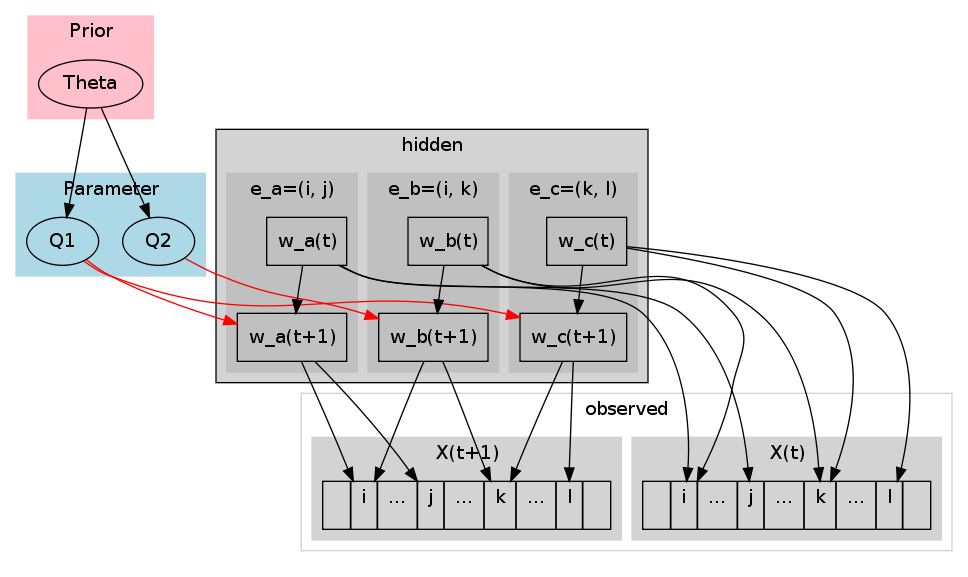
\includegraphics[scale=0.23]{images/factorial2}}
  \caption{Single functional classification model. Here, the
    edges $a, \,c$ belong to evolution class $1$, while edge $b$
    belongs to evolution class $2$. $X_{t}$ is the observed gene
    expression level at time $t$; $w_{e}(t)$ is the hidden variable
    denoting interaction strength for edge $e$ at time $t$; $Q_{i}$
    are the evolution characteristic for class $i$; and $\theta$ is
    the prior based on domain knowledge.}
  \label{fig:factorial}
\end{figure}

We use the factorial approximation where the parameter to be learnt is
the transition matrix $Q_{e}$ for each edge, $e = (i, j) \in E$.  We solve the Expectation
Maximization~(EM)\citep{Dempster77em} for MAP problem for each edge,
$e$,
\begin{equation}
  \label{eq:q-edge_em_map}
  \begin{array}[h]{llll}
  \textrm{E-step:} & {\mathcal L}(Q_{e}; Q_{e}^{(n)}) &=&
  E_{w_{e}^{|} }  [ \ln P(\mathbf{x}_{e}^{1:S}(1:T),
  \mathbf{w}_{e}({1:T}) | Q_{e})] \\
\vspace{2 mm}
  \textrm{M-step:} & \hat{Q}_{e}^{(n+1)} &=& \arg\max_{Q_{e}} (\ln P(Q_{e}) +
  {\mathcal L}(Q_{e}; Q_{e}^{(n)} ) ) 
  \end{array}
\end{equation}
where $W^{|}_{e}$ is the conditioned variable, $w_{e}(1:T)|
\mathbf{x}_{e}^{1:S}(1:T), Q_{e}^{(n)}$ and $Q_{e}^{(n)}$ is the
MAP estimate for the transition probability, $Q_{e}$, at the $n^{th}$
iteration of the algorithm. 

%Often, there is domain knowledge available which can be incorporated
%in the form of prior distribution. For example, one may know that most
%of the edges are inactive about 50\% of the time.

%\subsubsection{Dirichlet prior}
\subsubsection{Bayesian Approach: } The small number of observation
points poses an additional challenge in the inference of the
transition probability, $Q_{e}$. We use a 
bayesian approach to alleviate this problem.
We model the transition probabilities matrices as dirichlet distributions,
such that  the prior on the transition probabilities matrix, $Q$, 
given the parameter, $\Theta$, is
\begin{eqnarray}
  \label{eq:q_prior}
  P(\vec{q}_{l} | \vec{\theta}_{l}) &\sim& Dir(q_{l1}, \ldots, q_{l\mathcal{W}} ;
  \theta_{l1},\ldots, \theta_{l\mathcal{W}}) \\
&=& \frac{1}{B(\vec{\theta}_{l})} \prod_{m=1}^{\mathcal{W}} q_{lm}^{\theta_{lm}-1}
\end{eqnarray}
where $\vec{\theta}_{l}=[\theta_{l1},\ldots,\theta_{l\mathcal{W}}]$ and
$B(\vec{\theta}_{l})$ is the multinomial beta
function~\citep{Gelman03bayesian}.

This leads to the update equation for the MAP estimate for transition
probabilities, $q(l,m)$, obtained by the maximization step in (\ref{eq:q-edge_em_map}) as
\begin{equation}
  \label{eq:q-update}
  q^{(n+1)}_{e}(l, m) = \frac{(\theta_{lm}-1) + \sum_{t=1}^{T-1} \xi^{t}_{e}(l,
    m) }{\sum_{m} (\theta_{lm} -1) + \sum^{T-1}_{t=1} \sum^{\mathcal
      W}_{m=1} \xi^{t}_{e}(l,m)}
\end{equation}
where $\xi^{t}_{e}(l,m)$ is defined in the appendix~\ref{sec:fact-model-deriv}.
% \subsubsection{Cluster Similarity: } 
% We can often group the network interactions into categories  based on
% domain knowledge about the functional classification of genes.  For
% example, one might model the genes that participate in sugar
% metabolism as one 
% component, while treating genes involved in DNA synthesis as another
% component.  This allows us a
% simplification that we need to  consider only evolution over the
% \emph{components}(or \emph{clusters}), $A_k$ of edges,  which are parameterized by the
% cluster transition, $Q_{k}$ for  cluster $A_k$. 

% Then, the update equations for the transition probability matrix,
% $Q_k$, for the cluster, $A_k$ are as follows,
% \begin{eqnarray}
%   \label{eq:cluster_update}
%   q_{k}^{(n+1)}(l, m)   &=& \frac{(\theta^{(k)}_{lm} -1) + \sum_{e \in A_k} \sum_{t=1}^{T-1} \xi^{t}_{e}(l,m)}{ (\theta^{(k)}_{ij} -1) + \sum_{e \in A_k} \sum_{t=1}^{T-1}
%    \sum_{m} \xi^{t}_{e}(l,m)} \nonumber \\
% \end{eqnarray}
% where $\theta^{(k)}$ is the dirichlet parameter matrix for cluster,
% $A_{k}$.

\subsubsection{Quality of approximation:} We now discuss the
relationship between the factorial approximation and the original problem.  
\begin{lemma}
The factorial weights assumption gives a rank-1 tensor approximation~\citep{Horn90}  to the global weight
transition probability.  
\end{lemma}
For example, if the interaction network consists of two edges having transition
probabilities $A = \{a_{ij}\}$
 %$Q_{a}= \left\{\begin{array}{cc}   a_{11} & a_{12} \\     a_{21} &
 %a_{22} \end{array}\right\}$ 
and $B$ respectively, the approximation to
the original matrix, $\hat{Q}$ is given as the kronecker product
\[ \hat{Q} = A \otimes B = \left[
  \begin{array}{cc}
    a_{11} B & a_{12} B \\
    a_{21} B & a_{22} B
  \end{array}
\right]
\]

We note that if the weights indeed evolve independently of each other
and we are given the edge transition probabilities
$Q_{e}$, the overall system transition probability, $\mathbf{Q}$, is
given as 
\[
\mathbf{Q} = Q_{1} \otimes Q_{2} \otimes \ldots \otimes Q_{E}
\]
In general, if there are $E$ edges with estimated transition
probability matrices, $\hat{Q}_{1}, \ldots, \hat{Q}_{E}$, we obtain the approximation, $\hat{\mathbf{Q}}$
\[
\hat{\mathbf{Q}} \simeq Q_{1} \otimes Q_{2} \otimes \ldots \otimes Q_{E}
\]
We discuss the quality of approximation in case the original
probability matrix $Q$ is a higher order tensor
elsewhere. Section~\ref{sec:validation} presents a comparison of
the results obtained using the factorial approximation 
vs the results using a standard HMM implementation. 

Figure~\ref{fig:factorial} shows the graphical model corresponding to
the known network model with cluster similarity. We present a method
of incorporating the information from multiple slightly perturbed
strains into the inference algorithm in the following section. 
 

% $P(\mathbf{w}^{s}(t+1) = \mathbf{w}_{t+1} |  \mathbf{w}^{s}(t) =
%   \mathbf{w}_{t}, \mathbf{w}^{s}(t-1) = \mathbf{w}_{t-1},
%   \ldots) = P\left(\mathbf{w}^{s}(t+1) = \mathbf{w}_{t+1} |  \mathbf{w}^{s}(t) =
%   \mathbf{w}_{t}\right)$ for each strain. 
% We denote $Q$ as the
% transition probability of strain, $s$, such that
% \begin{equation}
%   \label{eq:Q-s}
%   Q^{s}(l, m) = P(\mathbf{w}^{s}(t+1) = \mathbf{w}_{m} |  \mathbf{w}^{s}(t) =
%   \mathbf{w}_{l})
% \end{equation}

\subsection{Strain Damping}
\label{sec:strain-damping-model} 
We consider the problem of multiple strainds which are just slightly
altered versions of the networks where a few genes have been knocked out of the
network. Therefore, most of the network remains the same across
strains with only the ``close'' neighbourhood of the knocked out genes
being affected. Thus, if one looks at a ``far'' edge,
$e_{far}$, the activation strength, $w_{e_{far}}(t)$, should be the
same across strains  the gene expression data for the edge strains,
$x^{1:S}_{e_{far}}(t)$, should be like i.i.d. samples, generated with
the same activation strength, $w_{e_{far}}(t)$. In the following discussion, 
we present a heuristic method which incorporates the ideas mentioned
above into the inference problem. 

We assume that the weights corresponding to the reference strain
$\mathbf{w}(t)$ evolve according to a Markov law given by a matrix $Q$,
where $Q(l, m) = P(\mathbf{w}(t+1) = \mathbf{w}_{m} | {\mathbf w}(t)
= \mathbf{w}_{l})$ with the property that $\sum_{m} Q(l, m) = 1$ for
all the initial states $\mathbf{w}_{l}$. For other strains, we assume
that the corresponding values are just slightly perturbed; thus
\begin{equation}
  \label{eq:damping}
 w^s_e(t) = w_e(t) \Gamma^s_e
\end{equation}
The perturbing parameters $\Gamma^s_e$ are determined
deterministically from the underlying network $G$ by
\begin{equation}
  \label{eq:edge-damping}
\Gamma^s(i,j) = (1 - \gamma^s_i)(1 - \gamma^s_j)  
\end{equation}
where $\gamma^s_i \in [0,1]$ is a label determined by how far the gene
$i$ is in the underlying network to one of the genes knocked out in
strain $s$. We note that the deterministic nature of the damping
implies that all strains evolve similarly, i.e., $Q^{s} = Q\;
\forall \; s$. This allows us to incorporate the information for gene
expression levels in the different strains while learning the temporal
evolution characteristics. 

We compute the damping factor, $\gamma^s_i$, for the genes
as follows: If the gene, $i$, is knocked out in strain $s$, then we
label it as $\gamma^s_i=0$. Now, we diffuse the labels across the
graph  such that $\gamma^{s}_i = \frac{1}{d(i)} \beta
\sum_{j\in N(i)} \gamma_j^s$, i.e., the damping factor at a node is
the average of the damping factors at its neighbours.    

 Intutitively, while $\Gamma_e = 0$ for an edge 
directly incident to one of the knocked out genes, the perturbation
gradually damps out with distance from the knocked out gene and for
an edge $e$ far away from one of the knocked out genes, $\Gamma_e
\approx 1$. Sections~\ref{sec:validation} and
\ref{sec:synthetic-dataset} present an experimental validation of the
model.

The next section presents a model which incorporates the functional
hierachy of genes in the inference procedure. 

\subsection{Mixture Model}
\label{sec:mixture-model}
% Significant progress has been
% made towards identifying the functional roles of the genes, resulting
% in a heirarchical classification of genomes based on their functional
% roles~\citep{DBLP:journals/nar/MewesAHLP97}. 
This section presents our approach to incorporating the
  functional categories of genes in our analysis. Since, genes belong
  to multiple categories, a mixture model is a naturally suited model
  to handle the influence of multiple functional categories in the
  inference procedure. 
%We seek to incorporate
%this information in our inference algorithm. \textcolor{red}{EXPAND ON GENE CLUSTER}
This allows us to explore  the relationship between functional
categories and the temporal evolution characteristics of the genes
which fall in the same functional category.

We now define the problem concretely. There are $H$ possible gene
categories. Each gene can be a member of one or more hierarchical
classes, $\mathcal{C}=\{C_{1},\ldots , C_{H}\}$, where the
hierarchical class $C_{h}$ is characterized by evolution matrix,
$Q_{h}$. The evolution probability matrix, $Q_{e}$, for each edge,
$e\in E$, is given as 
\begin{equation}
  \label{eq:q-mixture}
  Q_{e} = \sum_{h=1}^{H} \alpha_{e,h} Q_{h}
\end{equation}
where $\alpha_{e,h}$ denotes the influence of hierarchical class
$C_{h}$ in the edge, $e$, such that $\sum_{h} \alpha_{e, h} = 1$
for all edges $e \in E$. We define the random variable
$\mathbf{y}^{1:T} = \{y_e^t\}$ for all edges, $e \in E$,  and times,
$t=\{1,\ldots, T\}$ where $y^t_e$
denotes the component from which the evolution characteristics are
chosen at time $t$ for edge $e$ such that the event $y_e^t = h$
implies that $P(w_e^{t+1}= w_m | w^t_e =w_l, y_e^t = h) = q_h(l, m)$.
% Let $\gamma_e^t(h)$ be the probability $P(y^t_e =h )$.

We now outline the expectation maximization procedure~\citep{Bilmes98agentle,Mclachlan97embook} which
iteratively learns the unknown quantity, $\Psi = \{Q_{h},
\alpha_{e,h}\}$, for $h \in {\mathcal H} = \{1,\ldots, H\}$ and $e \in
E$ where  $Q_{h}$ is the class evolution
probability matrix for class, $C_h$, and $\alpha_{e,h}$ is the mixing
proportion for  edge, $e$ and class $C_h$; and $\Omega =
\{\mathbf{y}^{1:T},\mathbf{w}^{1:T}\}$ is
the hidden variable.  Let $\Psi^{(n)} = \{\alpha^{(n)}_{e,h},
Q^{(n)}_h\}$ be the estimates at the $n^{th}$ iteration. Then, 
\begin{equation}
  \label{eq:q-edge-mixture-em}
  \begin{array}[h]{llll}
  \textrm{E-step:} & {\mathcal L}(\Psi; \Psi^{(n)}) &=&
  E_{\Omega^{|} }  [ \ln P(\mathbf{x}^{1:S}(1:T), \Omega({1:T}) | \Psi({1:T}))] \\
\vspace{2 mm}
  \textrm{M-step:} & \hat{\Psi}^{(n+1)} &=& \arg\max_{\Psi} (\ln P(\Psi) +
  {\mathcal L}(\Psi; \Psi^{(n)} ) ) 
  \end{array}
\end{equation}
where $\Omega^{|}$ is the conditioned variable $(\mathbf{w}^{1:T},
\mathbf{y}^{1:T} | \mathbf{x}^{1:S}(1:T),  \Psi^{(n)})$.
\subsubsection{Domain knowledge:}
We incorporate the effect of the functional classification of
genes on the mixture components,
$\vec{\alpha}_e$, for an edge, $e$, by using a dirichlet prior of the form:
\begin{eqnarray}
  \label{eq:hier-prior}
  P(\vec{\alpha}_e) &\sim& Dir(\alpha_{e,1},\ldots, \alpha_{e,H};
  \gamma_{e,1},\ldots, \gamma_{e,H}) 
\end{eqnarray}
with the prior parameter, $\gamma_{e,h}$, for the edge, $e=(i,j)$, of the
form 
\begin{equation}
  \label{eq:mixture-prior}
  \gamma_{e,h} = \Big\{ \begin{array}{ll}
                       \gamma_p & \textrm{if genes }  i \textrm{ or } j
                       \textrm{ in class } h \\
                       \gamma_o & \textrm{otherwise}
                       \end{array}
\end{equation}
The maximization step in (\ref{eq:q-edge-mixture-em}) can  be done
separately for $q_h(l,m)$ and $\alpha_{e,h'}$ independently. We use
the priors in (\ref{eq:q_prior}) and
(\ref{eq:hier-prior})-(\ref{eq:mixture-prior}), and the constraints in
(\ref{eq:mixture-q-constraint})-(\ref{eq:mixture-alpha-constraint}) to
obtain the following update equations:%\footnote{\textcolor{red}{can be expanded lagrangian partial derivative}}
\begin{eqnarray}
  \label{eq:mixture-alpha-update}
  \alpha_{e,h'}^{(n+1)} =&  \frac{(\gamma_{e,h'}-1) + \sum_{t=1}^{T-1} \sum_{l,m,h}\xi^{t}_{e}(l,
    m,h,h') }{\sum_{h'} (\gamma_{e,h'} -1) + \sum^{T-1}_{t=1}
    \sum_{l,m,h,h'} \xi^{t}_{e}(l,m,h,h')} & \\
\label{eq:mixture-q-update} 
q^{(n+1)}_h(l,m) =&  \frac{(\theta_{lm}-1) + \sum_e \sum_{t=1}^{T-1}\sum_{h'}\xi^{t}_{e}(l,
    m,h,h') }{\sum_{m} (\theta_{lm} -1) + \sum_e \sum^{T-1}_{t=1}
    \sum_{m,h'} \xi^{t}_{e}(l,m,h,h')} &
\end{eqnarray}
where $\xi^{t}_{e}(l,m,h,h')$ is defined in appendix~\ref{sec:mixt-model-deriv}.
% The expectation step requires computation of the likelihood term
% ${\mathcal L}(\Psi;\Psi^{(n)})$ which involves expectation over terms
% $\log (\sum_h \alpha_{e,h}q_{h}(l, m) )$. Following standard mixture
% model techniques~\citep{Bilmes98agentle},
% \begin{equation}
%   \label{eq:em-mixture-exp1}
%    A
% \end{equation}

% We define a random variable, $Y^t_e(l,m)$, such that if $Y^t_e(l,m) = h$
% then the probability $P(w^{t+1}_e = w_m | w^{t}_e = w_l) = q_h(l,
% m)$, i.e., the $h^{th}$ mixing component is active. Let
% $\beta^{t}_{e,h}(l,m)$ denote the probability of the event $Y^t_e(l,m)
% = h$, i.e., $\beta^{t}_{e,h}(l,m)=P(Y^t_e(l,m)= h)$ and $\sum_h
% \beta^t_{e,h}(l,m)=1$.

% \subsection{Model 2: Regularization for unknown network}
% % We consider the exponential random graph model proposed by 

% We use the laplacian prior for the weights as follows $P(w) =\frac{\beta}{2} \exp(-\beta
% ||w||_{1})$. We 
\end{methods}
\section{Experiments}
\label{sec:experiments}
We present the experiments performed on synthetic and actual datasets
in this section. We compare the factorial weights and the mixture
model against a standard implementation of HMM which learn
the evolution characteristic for the system jointly in
\ref{sec:validation} and present the results on a synthetic dataset in
\ref{sec:synthetic-dataset}.

We apply our algorithm to infer the interaction strengths for two
genetic network scenarios. We are interested in the edges which show
considerable change during the measured time points. Towards this end,
we compute the change score, $s(e)$, of an interaction strength $w_{e}(1:T)$ as follows
\begin{equation}
  \label{eq:change-score}
  s(e) = \frac{1}{T} \sum_{t=1}^{T-1} (w_{e}(t+1) - w_{e}(t))^{2} 
\end{equation}
We fit an exponential distribution to it and look at the weights
falling in the top-$5 \%$ tail of the distribution.  
\subsection{Validation}
\label{sec:validation}
We choose a synthetic graph with $N=5$ nodes (genes) and $H=10$ functional
classes. The small value of $N$ allows direct estimation of the
transition probability matrix, $Q$,  of size ${\mathcal W}^{N} \times {\mathcal W}^{N}$,
using an standard implementation of
HMM\footnote{http://people.cs.ubc.ca/~murphyk/Software/HMM/hmm.html}.

The genes are randomly assigned classes  such that each
node is a member of $N_{av}=1.5$ classes on average. The weights take
possible values in ${\mathcal W} = \{-1, 1\}$, and the evolution characteristic, $Q_{e}$ for
each weight is a mixture based on the interacting genes.  We compare
the rank-1 approximations to the transition probability matrix of the
original HMM, $\hat{Q}_{large}$,  obtained by our methods to the
estimated transition probability matrix obtained from standard implementation of 
HMM for $N=20$ random trials. 

Figure~\ref{fig:validation-t} shows the comparison between different
methods with increasing length of the sequence, $T$. We note that the
standard HMM requires longer sequences to get comparable results with
factorial and mixture model approach. Figure~\ref{fig:validation-s} compares the
methods with increasing number of strains present (with at most 1 gene
knocked out). We note that the performance of the factorial weights
assumption shows a slight improvement with increasing number of
strains. 
\begin{figure}[h]
  \centering
  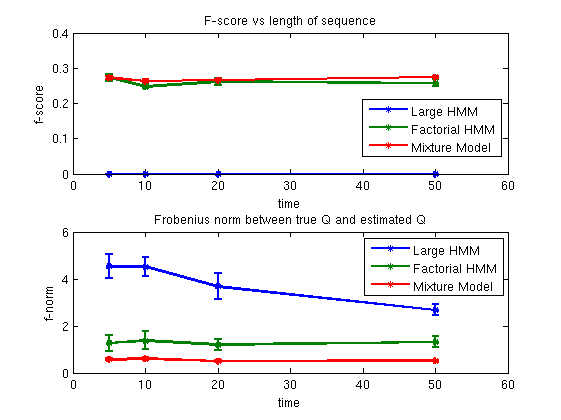
\includegraphics[scale=0.6]{results/mm_tvar}
  \caption{(a) F-score for the estimated weight evolution vs the true
    weight evolution sequence with increasing length of sequence, $T$. (b) Frobenius norm of the difference between the true
    evolution characteristics for the system and the estimated characteristics. }
  \label{fig:validation-t}
\end{figure}

\begin{figure}[h]
  \centering
  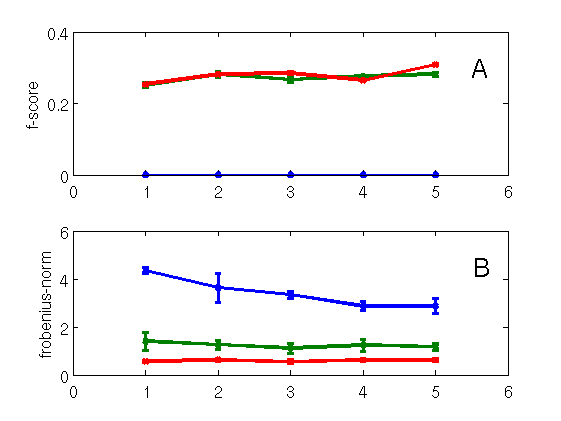
\includegraphics[scale=0.6]{results/mm_strain}
  \caption{(a) F-score for the estimated weight evolution vs the true
    weight evolution sequence with increasing number of strains. (b)
    Frobenius norm of the difference between the true evolution
    characteristics for the system and the estimated characteristics. } 
  \label{fig:validation-s}
\end{figure}


\subsection{Synthetic dataset}
\label{sec:synthetic-dataset}
% We consider a stochastic process $X(t) = \{x^1(t), \ldots, x^n(t)\}$
We generate a ``random'' graph $G=(V, E)$ with $C$ major components,
$\{A_1,\ldots, A_C\}$ with input parameters $p_{i}$ and $p_{c}$,
where $p_{i}$ is the probability, of an edge between two vertices in
the same component,  and $p_c$ is the probability of an edge between
two vertices in different components.  
%Each component has a transition probability matrix, $Q_c$, such that 

The activation level, $w_e(t)$ defined on an edge, $e$, belonging to
component, $A_k$, is a markov chain with transition probability matrix
$Q_{k}$. The problem is the estimation of the unknown transition probability
matrices $Q_k$ for each component, $A_k$. 

We use a noisy dirichlet prior for the estimation as follows: 
\begin{equation}
  \label{eq:exp1_prior}
\Theta^{(k)}  = Q_{k} + {\mathcal N}(0, \sigma^{2} I)   
\end{equation}
The experiment is conducted for $20$ trials with a graph of size
$N=50$ and number of components, $C$ chosen randomly between $2$ and
$10$. Figure~\ref{fig:exp1_fig} shows the F-scores for the
experiments done with multiple number of strains. 
% Figures~\ref{fig:exp1_fig} (b) shows the F-scores for the
% experiments with 2 strains with increasing number of missing gene.
 \begin{figure}[h]
   \centering
     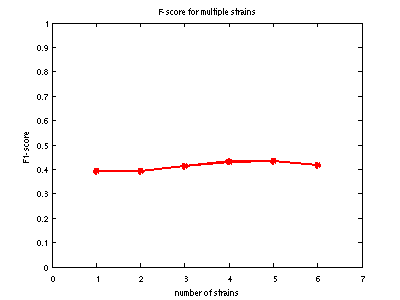
\includegraphics[scale=0.75]{results/Fig1_2}
%     & 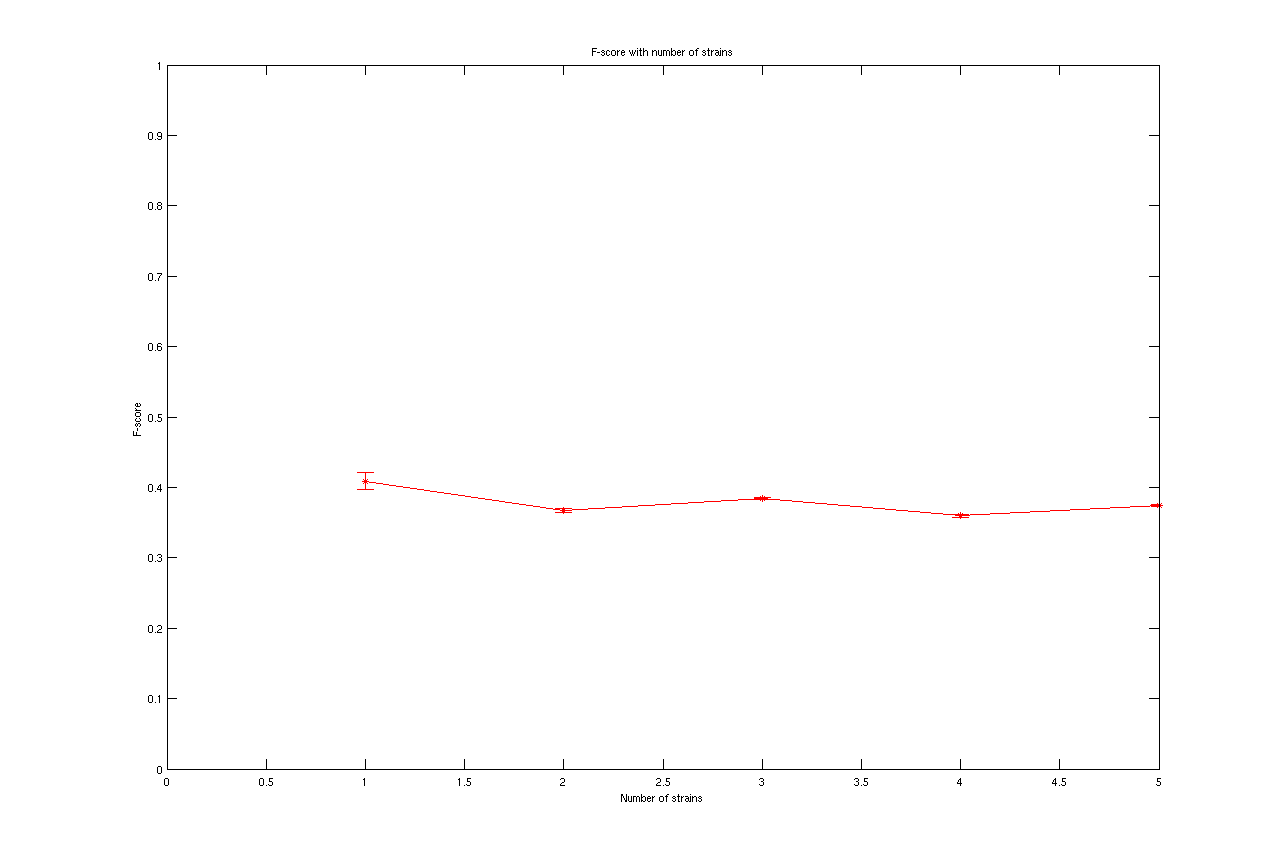
\includegraphics[scale=0.25]{results/f_score} \\
%     (a) & (b) 
%   \end{tabular}
   \caption{F-score for the synthetic dataset for multiple strains. We
     observe that increase in the number of strains provides more
     information about the activation strengths in the original
     network, which is visible in the slight increase in the
     F1-scores. However, since genes are being knocked out in each of
     the strains, the expression levels over multiple strains  are not equivalent to i.i.d. samples.  
   }
   \label{fig:exp1_fig}
 \end{figure}
\todo{BETTER NAMES NEEDED FOR EXPERIMENTS}
\subsection{Experiment 1}
\label{sec:experiment-1}

\subsection{Experiment 2}
\label{sec:experiment-2}
We run an experiment on \todo{[BIO EXPLANATION]}.  There are $S=2$
strains and $6$ time points $T=\{0, 5, 10, 30, 60, 120\}$ at which
expression level measurements were made. We analyze the the two
strains separately and then do a interaction network recovery for both
the strains using the strain damping model.

 
\section{Conclusion}
\label{sec:conclusions}

There is a tradeoff between using more sophisticated conditional
probability models $p(\mathbf{w}^{s}(t) |\mathbf{w}^{0}(t))$ involving more
parameters to be learnt and the limited amount of experimental
data. 


\bibliographystyle{bioinformatics}
\bibliography{default}
\appendix
% \section{Appendix}
% \subsection{Edge HMM}
% This section presents the derivation for the forward backward
% algorithm~\citep{Rabiner89hmm} under the factorial assumption for weights. 
% % We need to compute ${\mathcal L}(Q_{e};
% % Q_{e}^{n})$ in (\ref{eq:q-edge_em_map}), independently for each edge,
% % $e=(i,j)\in E$. This requires computing the conditional probability,
% % $P(\mathbf{w}_{e}^{1:T}| \mathbf{x}_{e}^{1:T}, Q_{e}^{(n)})$. 
% % We now outline the standard technique for parameter estimation in the
% % HMM~\citep{Rabiner89hmm} for the edge transition probabilities. 
%  The forward and the backward variables are defined as:
% \begin{eqnarray}
%   \label{eq:fwd}
%   f^{t}_{e}(l) &=& P(x_{e}^{1:S}(1:t) , w_{e}(t) = w_{l} | Q^{(n)}_{e}) \\
%   b^{t}_{e}(l) &=& P(x^{1:S}_{e}((t+1):T) | w_{e}(t) = w_{l}, Q^{(n)}_{e}) 
% \end{eqnarray}
% We assume that the data for strain, $s$, is independently generated based on the
% Ising model in (\ref{eq:ising}) with the weights that are damped
% versions (\ref{eq:edge-damping}) of the weights in the original
% strain. This leads to the observation model specified as:
% \begin{eqnarray}
%   \label{eq:obs}
%   o^{t}_{e}(l) &=& P(x_{e}^{1:S}(t) | w_{e}(t) = w_{l}) \\
% & = & \frac{1}{Z} \prod_{s=1}^{S} P(x_{e}^{s}(t) | w_{e}(t) = w_{l}) \\
% & = & \frac{\exp\left\{ - w_{l}\big(\sum_{s=1}^{S}
%       x^{s}_{i}(t)x^{s}_{j}(t) \Gamma^{s}(i,j)\big)
%   \right\}}{\sum^{\mathcal W}_{l=1}\exp\left\{ - w_{l}\big(\sum_{s=1}^{S}  x^{s}_{i}(t)x^{s}_{j}(t) \Gamma^{s}(i,j)\big) \right\}}
% \end{eqnarray}
% The update equations for computing the forward and backward variables
% are given as:
% \begin{eqnarray}
%   \label{eq:update}
%   f^{t+1}_{e}(m) &=& P(x_{e}^{1:S}(1:t) , w_{e}(t) = w_{l} | Q^{(n)}_{e}) \\
% o^{t+1}_{e}(m) \sum_{l=1}^{{\mathcal W}} f_{e}^{t}(l) q_{e}^{(n)}(l, m) \\
%   b^{t}_{e}(l) &=& P(x^{1:S}_{e}((t+1):T) | w_{e}(t) = w_{l}, Q^{(n)}_{e}) 
% \sum_{m=1}^{{\mathcal W}} q_{e}^{(n)}(l, m) o^{t+1}_{e}(m) b^{t+1}_{e}(m)
% \end{eqnarray}
% and the joint probability, $\xi_{e}^{t}(l,m)=P(w_{e}(t) =
% w_{l}, w_{e}(t+1) = w_{m} | x^{1:S}_{e}(1:T), Q^{(n)}_{e})$, is given as follows:
% \begin{eqnarray}
%   \label{eq:p-joint}
%   \xi_{e}^{t}(l,m) &=& \frac{f_{e}^{t}(l) q_{e}^{(n)}(l, m)
%     o_{e}^{t+1}(m) b^{t+1}(m)}{P(x^{1:S}(1:T) | Q^{(n)}_{e})} \\
% &=& \frac{f_{e}^{t}(l) q_{e}^{(n)}(l, m)
%     o_{e}^{t+1}(m) b^{t+1}(m)}{
%     \sum_{l, m} f_{e}^{t}(l) q_{e}^{(n)}(l, m)
%     o_{e}^{t+1}(m) b^{t+1}(m) }
% \end{eqnarray}

\appendix
\section{Factorial model derivation}
\label{sec:fact-model-deriv}
This section presents a derivation of the forward and backward
probabilities with the strain damping model. We assume that the data
for strain, $s$, is independently generated 
based on the Ising model in (\ref{eq:ising}) with the weights that are
damped versions (\ref{eq:damping}) of the weights in the original 
strain. This leads to the observation model specified as:
\begin{eqnarray}
  \label{eq:obs}
  o^{t}_{e}(l) &=& P(x_{e}^{1:S}(t) | w_{e}(t) = w_{l}) \\
\label{eq:obs2}
& = & \frac{1}{Z} \prod_{s=1}^{S} P(x_{e}^{s}(t) | w_{e}(t) = w_{l})
\\
\label{eq:obs3}
& = & \frac{\exp\left\{ - w_{l}\big(\sum_{s=1}^{S}
      x^{s}_{i}(t)x^{s}_{j}(t) \Gamma^{s}(i,j)\big)
  \right\}}{\sum^{\mathcal W}_{l=1}\exp\left\{ - w_{l}\big(\sum_{s=1}^{S}  x^{s}_{i}(t)x^{s}_{j}(t) \Gamma^{s}(i,j)\big) \right\}}
\end{eqnarray}
If the strains are all identical (Section~\ref{sec:factorial-model}),
then, the observations $x^{s}_{i}(t)$ can be considered as
i.i.d. samples, i.e., the damping factor $\Gamma^{s}(i,j) = 1$ for all
$i, j$. 
The update equations for computing the forward and backward
probability distributions are given as:
\begin{eqnarray}
  \label{eq:update}
  f^{t+1}_{e}(m) &=& P(x_{e}^{1:S}(1:t) , w_{e}(t+1) = w_{m} | Q^{(n)}_{e}) \\
&=& o^{t+1}_{e}(m) \sum_{l=1}^{{\mathcal W}} f_{e}^{t}(l) q_{e}^{(n)}(l, m) \\
  b^{t}_{e}(l) &=& P(x^{1:S}_{e}((t+1):T) | w_{e}(t) = w_{l},
  Q^{(n)}_{e})  \\
\label{eq:update-1}
&=& \sum_{m=1}^{{\mathcal W}} q_{e}^{(n)}(l, m) o^{t+1}_{e}(m) b^{t+1}_{e}(m)
\end{eqnarray}
and the joint probability as
\begin{eqnarray}
  \label{eq:p-joint}
  \xi_{e}^{t}(l,m) &=& P(w_{e}(t,t+1) =(w_{l}, w_{m}) |
  x^{1:S}_{e}(1:T), Q^{(n)}_{e}) \\
&\propto& f_{e}^{t}(l) q_{e}^{(n)}(l, m) o_{e}^{t+1}(m) b^{t+1}(m) 
\end{eqnarray}

\section{Mixture model derivation}
\label{sec:mixt-model-deriv}
%The factorial approximation in the previous section allows us to
%compute the probability distribution over the edges independently.
% The edge evolution matrix, $Q^{(n)}_e$ is given as: 
% \begin{equation}
%   \label{eq:q-e-mixture}
%   q_e^{(n)}(l,m) = \sum_{h=1}^H \alpha^{(n)}_{e,h} Q^{(n)}_h(l,m)
% \end{equation}
% \begin{remark}[VJ: ]
% \end{remark}
This section presents the derivation for the forward and backward
probability distributions in the mixture model. The observation model, $o^t_e(l)=P(x^{1:S}_e(t) | w^t_e=w_l)$ , remains unchanged as in
(\ref{eq:obs})-(\ref{eq:obs3}). 
%The forward iterates, $f_e^{t}(m)$, and the backward iterates,
%$b^t_e(m)$, remain unchanged as in (\ref{eq:update})-(\ref{eq:update-1}). 
The forward iterates, $f_e^t(l, h)$ and backward iterates, $b_e^t(l,
h)$ can  be computed as follows: 
\begin{eqnarray}
  \label{eq:mixture-update}
  f^{t}_{e}(m, h) &=& P(x_{e}^{1:S}(1:t) , w_{e}^{t} = w_{m},
  y_e^t = h | \Psi^{(n)}_{e}) \\
&=& P(x^{1:S}_e(t) | w_m) \sum_{w_l} \sum_{h'}
\Big[ P(y^t_e=h | \alpha^{(n)})  \nonumber \\
&\times& P(w_m | w^{t-1}_e = w_l, y^{t-1}_e = h')  \times f_e^{t-1}(l, h')
\Big]\\
%% final forward equation
&=& o^{t}_{e}(m) \sum_{l=1}^{{\mathcal W}} \sum_{h'=1}^H
f_{e}^{t-1}(l, h') \alpha_h^{(n)} q_{h'}^{(n)}(l, m) \\
%% backward equations
  b^{t}_{e}(m, h) &=& P(x^{1:S}_{e}((t+1):T) | w_{e}(t) = w_{m}, y_e^{t}=h,
  \Psi^{(n)}_{e})  \\
&=&  \sum_{w_l} \sum_{h'} \Big[ P(x^{1:S}_e(t+1) | w^{t+1}_e = w_l)
  b_e^{t+1}(l, h')\nonumber \\
&\times& P(w^{t+1}_e = w_l | w_m, y^{t}_e = h)   P(y^{t+1}_e=h' | \alpha^{(n)}) 
\Big]\\
%% final backward equation
\label{eq:mixture-update-1}
&=& \sum_{m=1}^{{\mathcal W}}\sum_{h'=1}^H q_{h}^{(n)}(m, l) o^{t+1}_{e}(l) \alpha^{(n)}_{h'}b^{t+1}_{e}(l,h')
\end{eqnarray}
The conditional probability $P(\Omega_e^{t}=(w_l, h), \Omega_e^{t+1}
=(w_m, h') | \mathbf{x}_e^{1:S}(1:T) , \Psi^{(n)})$ denoted by $\xi^t_e(l,m,h,h') $ can be computed as
\begin{equation}
  \label{eq:mixture-p-cond}
  \xi^t_e(l,m,h,h') \propto f^t_e(l,h)\alpha_{h'}^{(n)} q^{(n)}_h(l,m)
  o^{t+1}_e(m) b_e^{t+1}(m, h')
\end{equation}
The likelihood term, $ {\mathcal L}(\Psi; \Psi^{(n)})$, in (\ref{eq:q-edge-mixture-em}) can be expressed
in terms of the conditioned edge probabilities, $\xi^t_e$, in
(\ref{eq:mixture-p-cond}) as 
\begin{eqnarray}
  \label{eq:mixture-L-edge}
  {\mathcal L}(\Psi; \Psi^{(n)}) &=& \sum_{e\in E}\sum_{t=1}^{T-1}
  \mathbf{E}_{\xi^t_e}[\ln q_h(l, m) + \ln \alpha_{e,h'}]
\end{eqnarray}
subject to the constraints
\begin{eqnarray}
  \label{eq:mixture-q-constraint} \sum_{m} q_h(l,m) &=& 1 \quad\forall h \\
   \label{eq:mixture-alpha-constraint} \sum_{h} \alpha_{e,h} &=& 1 \quad\forall e
\end{eqnarray}


\end{document}